\documentclass[
	% -- opções da classe memoir --
	article,			% indica que é um artigo acadêmico
	11pt,				% tamanho da fonte
	oneside,			% para impressão apenas no recto. Oposto a twoside
	a4paper,			% tamanho do papel.
	% -- opções da classe abntex2 --
	%chapter=TITLE,		% títulos de capítulos convertidos em letras maiúsculas
	%section=TITLE,		% títulos de seções convertidos em letras maiúsculas
	%subsection=TITLE,	% títulos de subseções convertidos em letras maiúsculas
	%subsubsection=TITLE % títulos de subsubseções convertidos em letras maiúsculas
	% -- opções do pacote babel --
	english,			% idioma adicional para hifenização
	brazil,				% o último idioma é o principal do documento
	sumario=tradicional
	]{abntex2}


% ---
% PACOTES
% ---

% ---
% Pacotes fundamentais
% ---
\usepackage{lmodern}			% Usa a fonte Latin Modern
\usepackage[T1]{fontenc}		% Selecao de codigos de fonte.
\usepackage[utf8]{inputenc}		% Codificacao do documento (conversão automática dos acentos)
\usepackage{indentfirst}		% Indenta o primeiro parágrafo de cada seção.
\usepackage{nomencl} 			% Lista de simbolos
\usepackage{color}				% Controle das cores
\usepackage{graphicx}			% Inclusão de gráficos
\usepackage{float}
\usepackage{microtype} 			% para melhorias de justificação
\usepackage{quoting}
% ---

% ---
% Pacotes de citações
% ---
\usepackage[brazilian,hyperpageref]{backref}	 % Paginas com as citações na bibl
\usepackage[alf]{abntex2cite}	% Citações padrão ABNT
% ---

% ---
% Configurações do pacote backref
% Usado sem a opção hyperpageref de backref
\renewcommand{\backrefpagesname}{Citado na(s) página(s):~}
% Texto padrão antes do número das páginas
\renewcommand{\backref}{}
% Define os textos da citação
\renewcommand*{\backrefalt}[4]{
	\ifcase #1 %
		Nenhuma citação no texto.%
	\or
		Citado na página #2.%
	\else
		Citado #1 vezes nas páginas #2.%
	\fi}%
% ---

% ---
% Informações de dados para CAPA e FOLHA DE ROSTO
% ---
\titulo{Relatório de trabalho no OrchFlow}
\autor{
	Angelo Silva \thanks{angelorodriigo.rs@gmail.com}
	\and Dante Mesquita Neto \thanks{dantemesquitaneto@gmail.com}
	\and Jônatas Bonventti \thanks{jonatasbvt@yahoo.com}
	\and Pedro \thanks{pedro\_vkf@hotmail.com}
}
\local{Brasil}
\data{2018, v-1.0.0}
% ---

% ---
% Configurações de aparência do PDF final

% alterando o aspecto da cor azul
\definecolor{blue}{RGB}{41,5,195}

% informações do PDF
\makeatletter
\hypersetup{
     	%pagebackref=true,
		pdftitle={\@title},
		pdfauthor={\@author},
    	pdfsubject={Relatório de trabalho em cima do OrchFlow},
	    pdfcreator={LaTeX with abnTeX2},
		pdfkeywords={orchflow}{controladores}{java}{neo4j}{redes},
		colorlinks=true,       		% false: boxed links; true: colored links
    	linkcolor=blue,          	% color of internal links
    	citecolor=blue,        		% color of links to bibliography
    	filecolor=magenta,      		% color of file links
		urlcolor=blue,
		bookmarksdepth=4
}
\makeatother
% ---

% ---
% compila o indice
% ---
\makeindex
% ---

% ---
% Altera as margens padrões
% ---
\setlrmarginsandblock{3cm}{3cm}{*}
\setulmarginsandblock{3cm}{3cm}{*}
\checkandfixthelayout
% ---

% ---
% Espaçamentos entre linhas e parágrafos
% ---

% O tamanho do parágrafo é dado por:
\setlength{\parindent}{1.3cm}

% Controle do espaçamento entre um parágrafo e outro:
\setlength{\parskip}{0.2cm}  % tente também \onelineskip

% Espaçamento simples
\SingleSpacing

% ----
% Início do documento
% ----
\begin{document}

% Seleciona o idioma do documento (conforme pacotes do babel)
%\selectlanguage{english}
\selectlanguage{brazil}

% Retira espaço extra obsoleto entre as frases.
\frenchspacing

% ----------------------------------------------------------
% ELEMENTOS PRÉ-TEXTUAIS
% ----------------------------------------------------------

%---
%
% Se desejar escrever o artigo em duas colunas, descomente a linha abaixo
% e a linha com o texto ``FIM DE ARTIGO EM DUAS COLUNAS''.
% \twocolumn[    		% INICIO DE ARTIGO EM DUAS COLUNAS
%
%---
% página de titulo
\maketitle

% resumo em português
\begin{resumoumacoluna}
  Durante manutenção no orquestrador java OrchFlow, viu-se a necessidade da refatoração em cima da implementação existente. Pontos de mudança com alto acoplamento foram trabalhados para, futuramente, proporcionar mais facilidade na hora de incrementar a aplicação e apliar correção de erros.

 \vspace{\onelineskip}

 \noindent
 \textbf{Palavras-chave}: neo4j. controladores. java. floodlight.
\end{resumoumacoluna}

% ]  				% FIM DE ARTIGO EM DUAS COLUNAS
% ---

% ----------------------------------------------------------
% ELEMENTOS TEXTUAIS
% ----------------------------------------------------------
\textual

% ----------------------------------------------------------
% Introdução
% ----------------------------------------------------------
\section*{Introdução}
\addcontentsline{toc}{section}{Introdução}

Devido a tomadas de decisão imaturas, partes do software acabaram ao longo da primeira implantação do sistema levando um rumo não focado em qualidade, mas sim em simplesmente finalizar a implantação.
Através de técnicas simples de desenvolvimento de software e devops, tentamos reescrever pequenos trechos da aplicação, refatorando o sistema.

\section{Mudanças implementadas}

\subsection{Docker e contêineres}

Para melhor acolhermos os desenvolvedores da plataforma, utilizamos contêineres linux sendo gerenciados por docker e docker-compose para conseguirmos rodar a aplicação, conseguimos controlar partes do software dentro de contêineres mas outras não, floodlight e mininet foram duas dependências que não puderam ser controladas de forma separada a tempo da entrega do projeto.

A arquitetura final dos contêineres ficou como descrito na figura \ref{figure_arquitetura_container}.

\begin{figure}[H]
    \label{figure_arquitetura_container}
    \centering
    \caption{Arquitetura dos contêineres}
    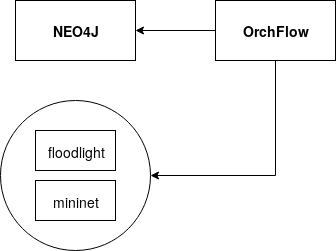
\includegraphics[scale=0.8]{arquitetura_container.png}
    \hfill
\end{figure}

\subsubsection{Contêiner neo4j}

O contêiner do neo4j fica responsável por manter uma instância do banco de dados, poderíamos trabalhar com um cluster de contêineres, mantendo diversas instâncias sendo controlada pelo docker-compose, aproveitando-se de benefícios como scaling e loadbalance.

\subsubsection{Imagem do floodlight com mininet}

O contêiner do floodlight com o mininet é onde o problema está, em um cenário de contêineres, cada um deve rodar apenas um serviço linux, porém, durante a definição dos contêineres, foram encontrados problemas de comunicação entre um contêiner floodlight e um mininet, portanto, uma imagem limpa e simples do mininet com floodlight foi mantida, por não fazer parte da aplicação OrchFlow, mas sim, ser um cliente.

\subsubsection{Contêiner do OrchFlow}

O contêiner do OrchFlow vai manter uma instância da aplicação rodando em uma imagem com base em java e tomcat, se comunicando com o contêiner do neo4j e da imagem do floodlight teste.

\subsubsection{Receptibilidade de desenvolvedores}

Implementando uma infraestrutura baseada em contêineres conseguimos reduzir consideravelmente a receptibilidade de novos programadores no projeto, como cada serviço fica contido dentro do seu próprio contêiner, configurar um ambiente de desenvolvimento se torna algo até mesmo monótono, não se perde mais tempo tentando entender configurações mágicas que, uma vez não documentadas, são esquecidas.

\subsection{Acoplamento de configurações}

Um outro problema que foi notado ao iniciar o projeto de manutenção do OrchFlow, que, somado a uma arquitetura baseada em contêineres poderia tornar o desenvolvimento mais rápido, é o acoplamento de configurações, existem chaves de API e configurações de banco de dados direto no código da aplicação, isso torna a arquitetura OrchFlow um impedimento para novos programadores.
Para solucionar o problema, criamos um pacote, centralizando todas as configurações do sistema.

\subsection{Padrões de nomeação}

Foi trabalhada durante a manutenção do sistema um novo padrão de nomeação, problemas com nomeação de classes e camadas foram solucionados, unificando o idioma para o inglês americano.

\subsection{Síndrome das janelas quebradas}

Durante o desenvolvimento do projeto, notamos um problema que acontece na maioria dos projetos de software, o projeto começa bem, com uma curva de trabalho e implementação altíssima, porém ao longo do tempo, conforme a base de código cresce, trechos de código ficam para trás no que toca cuidado e boas práticas.

\subsubsection{Padrão}

Padrões surgiram para trazer abertura para desenvolvedores, assim como a experiência do usuário, temos também a experiência do desenvolvedor ao trabalhar em um projeto, a partir do momento onde cada pessoa que escreve detalhes de implementação, o faz conforme imagina, temos um problema de pai, somente uma pessoa conhece como aquele pedaço de código funciona, por tal, durante a manutenção do projeto, foram discutidos padrões de desenvolvimento de software, desde a arquitetura do sistema até a indentação de parâmetros de um método.

\subsubsection{Comentários}

Segundo \citeonline[p. 51]{cleancode},

\begin{quoting}[rightmargin=0cm,leftmargin=4cm]
	{\footnotesize \noindent Nada por ser tão útil quanto um comentário bem colocado. Nada consegue amontoar um módulo mais do que comentários dogmáticos e supérfluos. Nada pode ser prejudicial quanto um velho comentário mal feito que dissemina mentiras e informações incorretas. }
\end{quoting}

Um comentário em um código tem uma série de problemas, um dos mais identificados dentro da base de código do OrchFlow foi código velho, código que por algum motivo estava sendo trabalhado e foi deixado para trás, isso trás dúvidas quanto os detalhes de implementação.

Muitas vezes um código está tão mal escrito, que muitos programadores desejariam um código em cima do comentário o explicando, se é necessário um comentário explicando como aquele código funciona, provavelmente o código não foi capaz de expressão sua intenção através de boa nomeação e estruturação.

\section{Mudanças futuras ou em andamento}

\subsection{Problemas na separação de camadas}

A grande dificuldade em manter o projeto está em sua arquitetura, a separação de camadas é feita de forma errônea, se comunicando diretamente com dados através das controllers, com regras de negócio no mesmo lugar.
Uma arquitetura que poderia solucionar o problema é separar as camadas e suas responsabilidades como descrito na figura \ref{figure_arquitetura_camadas}.

\begin{figure}[H]
    \label{figure_arquitetura_camadas}
    \centering
    \caption{Arquitetura de camadas}
    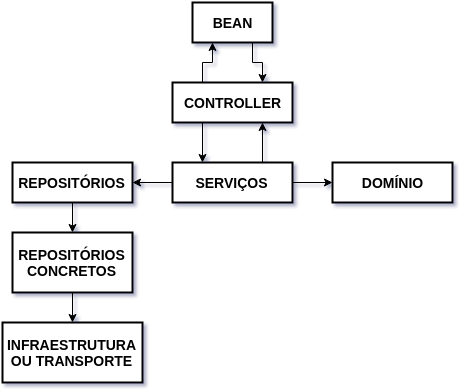
\includegraphics[scale=0.8]{arquitetura_camadas.png}
    \hfill
\end{figure}
{
\section{Bean}

Como não foi pensado sair da arquitetura padrão do OrchFlow, trocando para algum outro framework, foi decidido por manter os beans como um DTO, uma camada de transporte dos dados da aplicação até a View.
Na aplicação, os beans do Java simplesmente mantém os dados para serem trabalhados na view, eles se comunicam passando as informações para a controller, simulando uma requisição http.

\section{Controle}

A camada de controle, trabalha de forma a fazer uma validação básica, trabalhando normalmente em cima de tipos, verificando se a requisição possui todo os dados necessários.
Ela se comunica com os serviços da aplicação, requisitando os casos de uso.

\section{Domínio}

A camada de domínio é a mais importante dentro de uma aplicação, é nela que as regras de negócio estão inseridas, elas são utilizadas também como entidades, sendo passadas e retornadas pelos repositórios.

\section{Serviços}

Na camada de serviços, são implementados os casos de uso da aplicação, utilizando, podem ser colocadas nessa camada regras de validação de dados, ela se comunica com a camada de domínio da aplicação, chamando as regras de negócio e também com os repositórios na hora de se comunicar externamente.

\section{Repositórios}

A camada de repositório, se comunica com aplicações externas, é comum encontrarmos nessa camada, chamadas para persistência de dados, porém, podem ser serviços externos diferentes, como um API, um broker, banco de dados, entre diversos outros, é uma boa prática chamar nessa camada um repositório concreto, que possui comunicação com a camada de infraestrutura para o método de persistência desejado.

\section{Infraestrutura}

A camada de infraestrutura é a camada de comunicação, é nela que ficam as chamadas para os serviços externos da aplicação, a troca da infraestrutura de um usuário de banco de dados para uma chamada em uma API não deve alterar o funcionamento de outra camadas por exemplo.
Para se adequar ao OrchFlow, as chamadas a API do neo4j, por exemplo, poderiam ser implementadas aqui.

% ----------------------------------------------------------
% Referências bibliográficas
% ----------------------------------------------------------
\bibliography{abntex2-modelo-references}

\end{document}
